\paragraph{to add}
In addition to coreset sampling, we could also run on the whole feature, 

\section{Performance Measurements and Results}

\subsection{Performance metrics}
There are three common performance metrics, we have our own way to measure:
\begin{itemize}
    \item Execution time: one is run-time, the other is normalized instance hour;
    \item Memory-consumption \& number of machines: peak memory of mapper and reducer, see Table \ref{table:m3}. We use m3.2xlarge and one master, two cores.
    \item Solution quality: our project is quite innovative and there is no existing work. We can only compare our results with differnt parameters by topographical world map\cite{world}.
\end{itemize}

\begin{table}
    \centering
    \label{table:m3}
    \begin{tabular}{|l|l|l|l|}
        \hline
        Model & vCPU & Mem (GiB) & SSD Storage (GB) \\
        \hline
        m3.medium & 1 & 3.75 & 1 x 4  \\
        m3.large  & 2 & 7.5 & 1 x 32 \\
        m3.xlarge & 4 & 15 & 2 x 40 \\
        m3.2xlarge& 8 & 30 & 2 x 80 \\
        \hline
    \end{tabular}
\end{table}

\subsection{Result of recent four decades}
Same as Milestone $3$, we selected the year $1983$, $1993$, $2003$ and $2013$ to show the results. The size of raw compressed dataset is as showing in the Table \ref{4year}.

\begin{table}
    \centering
    \label{4year}
    \begin{tabular}{|l|l|l|l|}
        \hline
        1983 & 1993 & 2003 & 2013 \\
        \hline
        155M & 152M & 159M & 166M \\
        \hline
    \end{tabular}
\end{table}

We kept adjusting the parameters until we found the result is resonable. The following pictures is snapthots from 150 clusters, 500 iterations.

\begin{comment}
\begin{figure}
    \centering
    \begin{tabular}{c}
        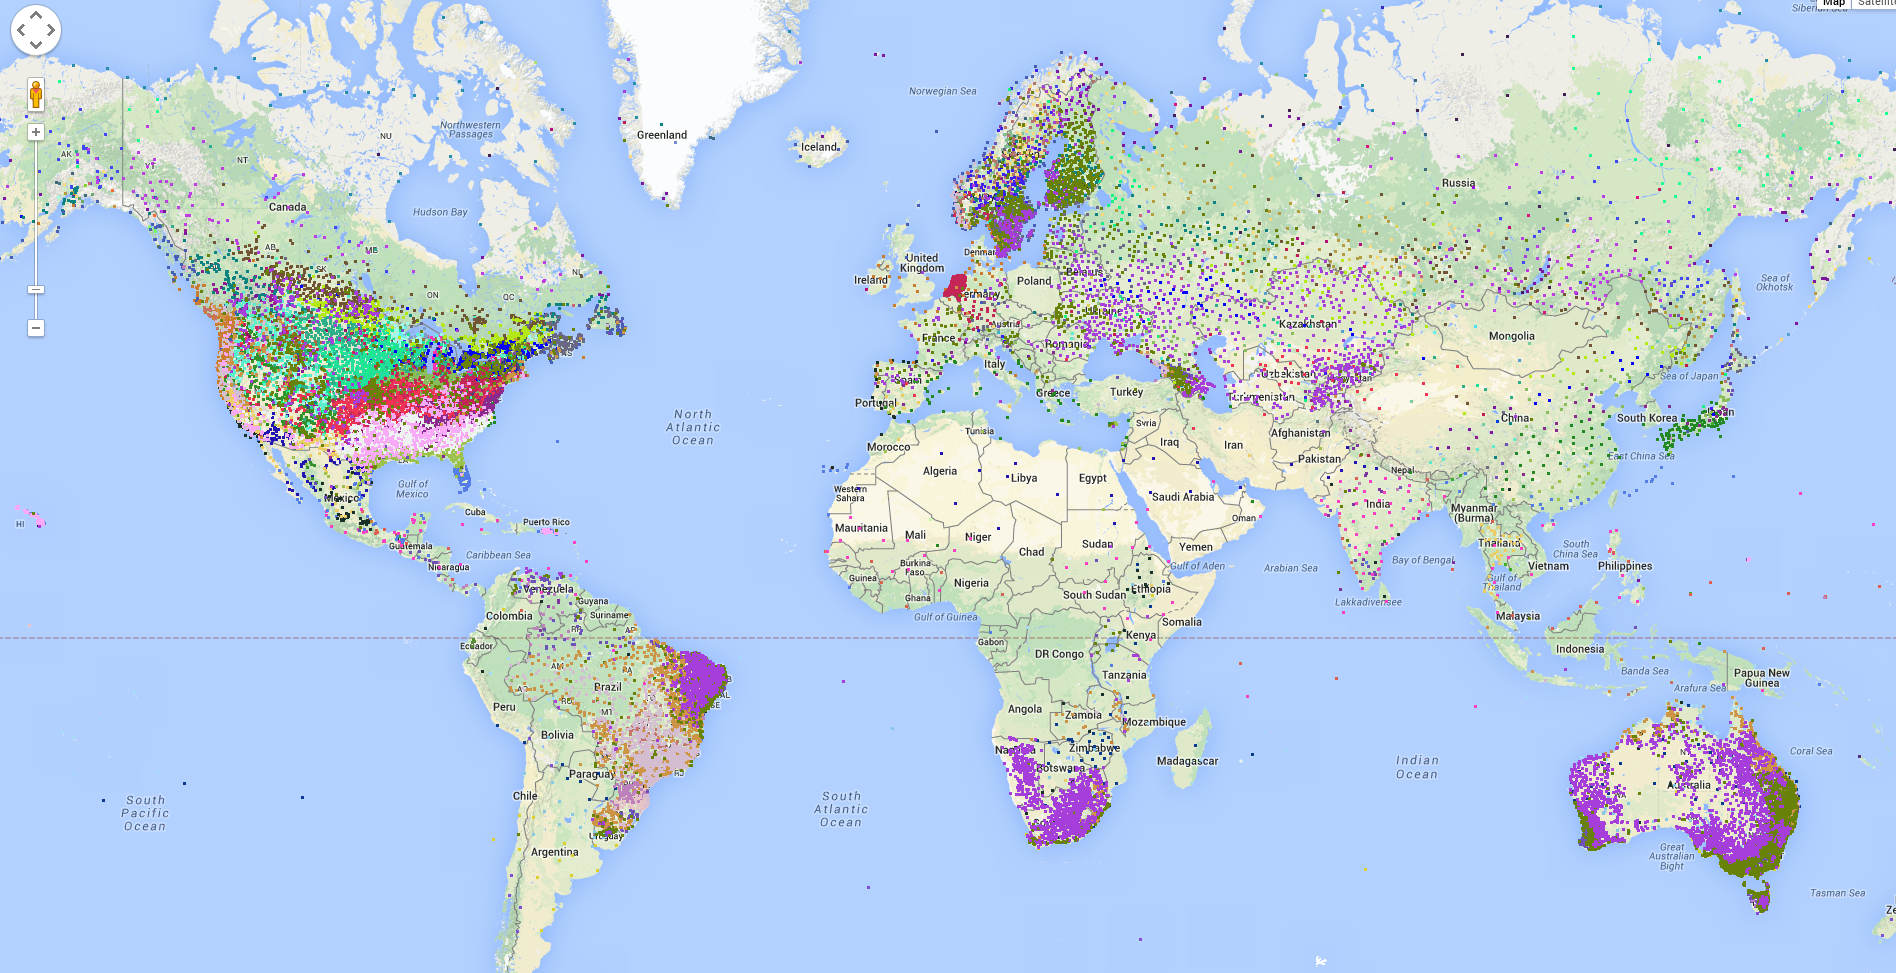
\includegraphics[width =\linewidth]{images/1983.png}\\1983\\
        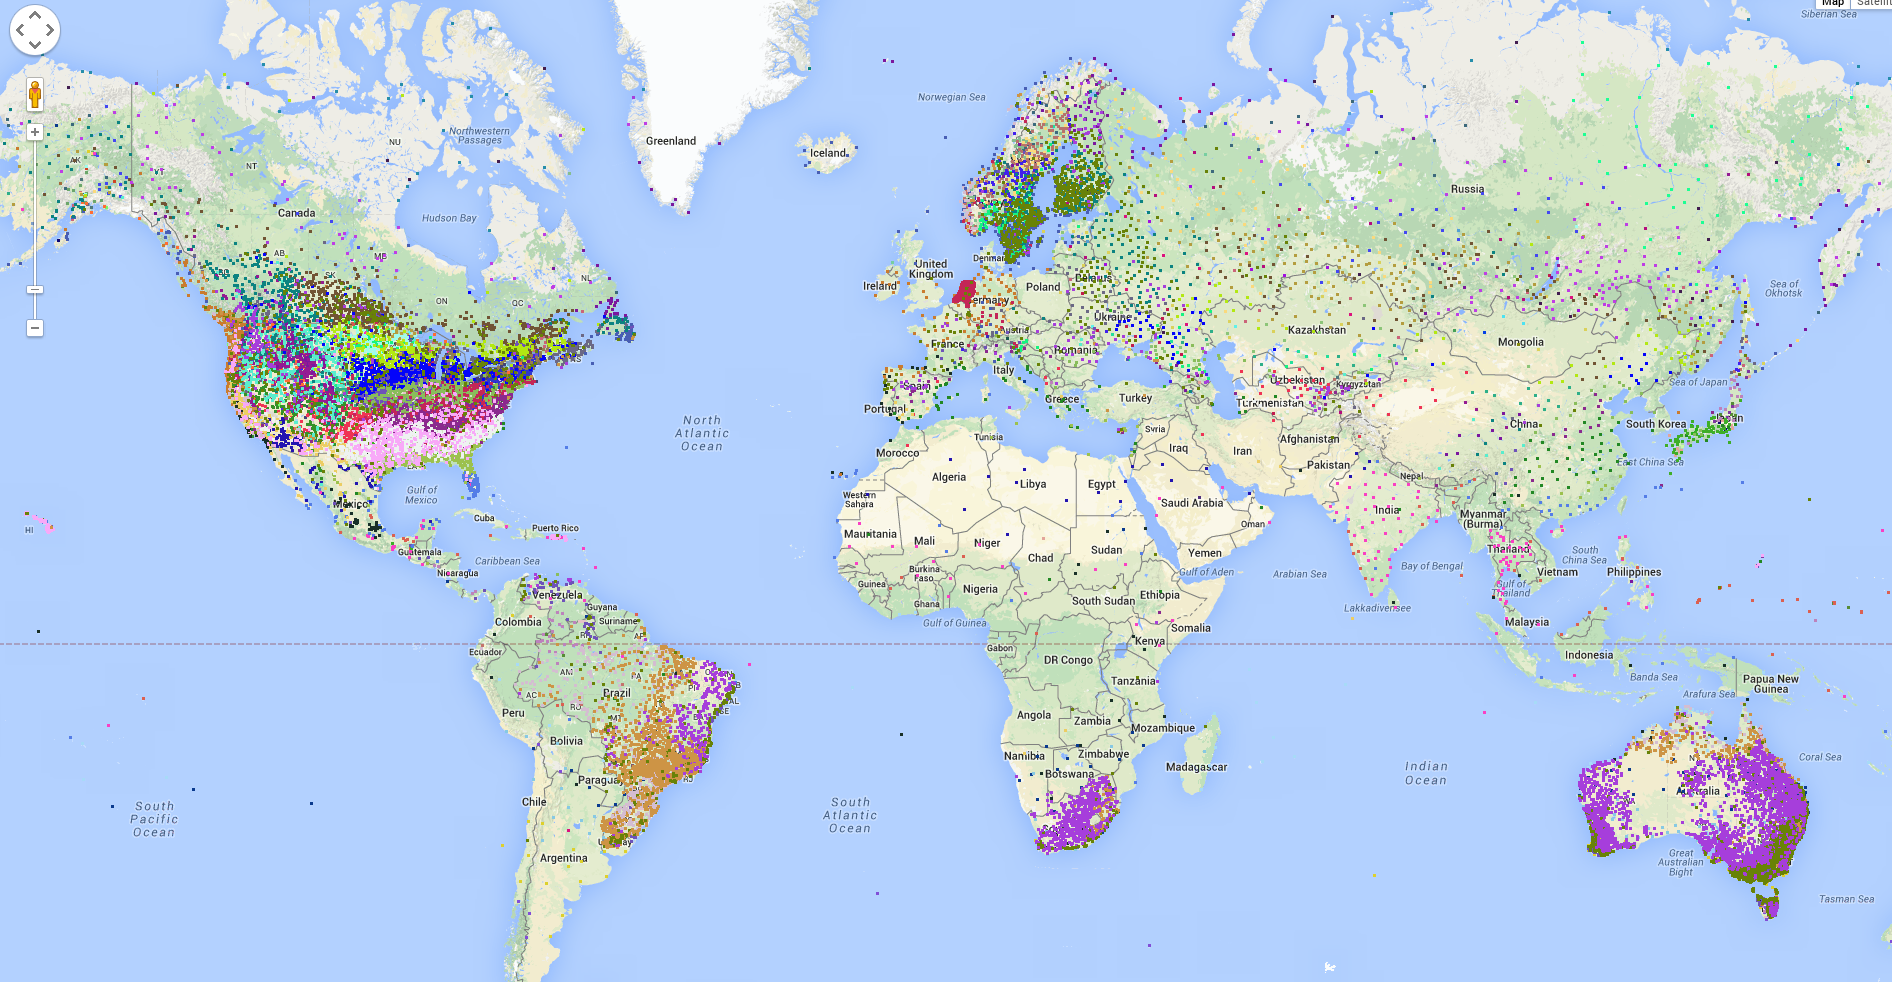
\includegraphics[width =\linewidth]{images/1993.png}\\1993\\
        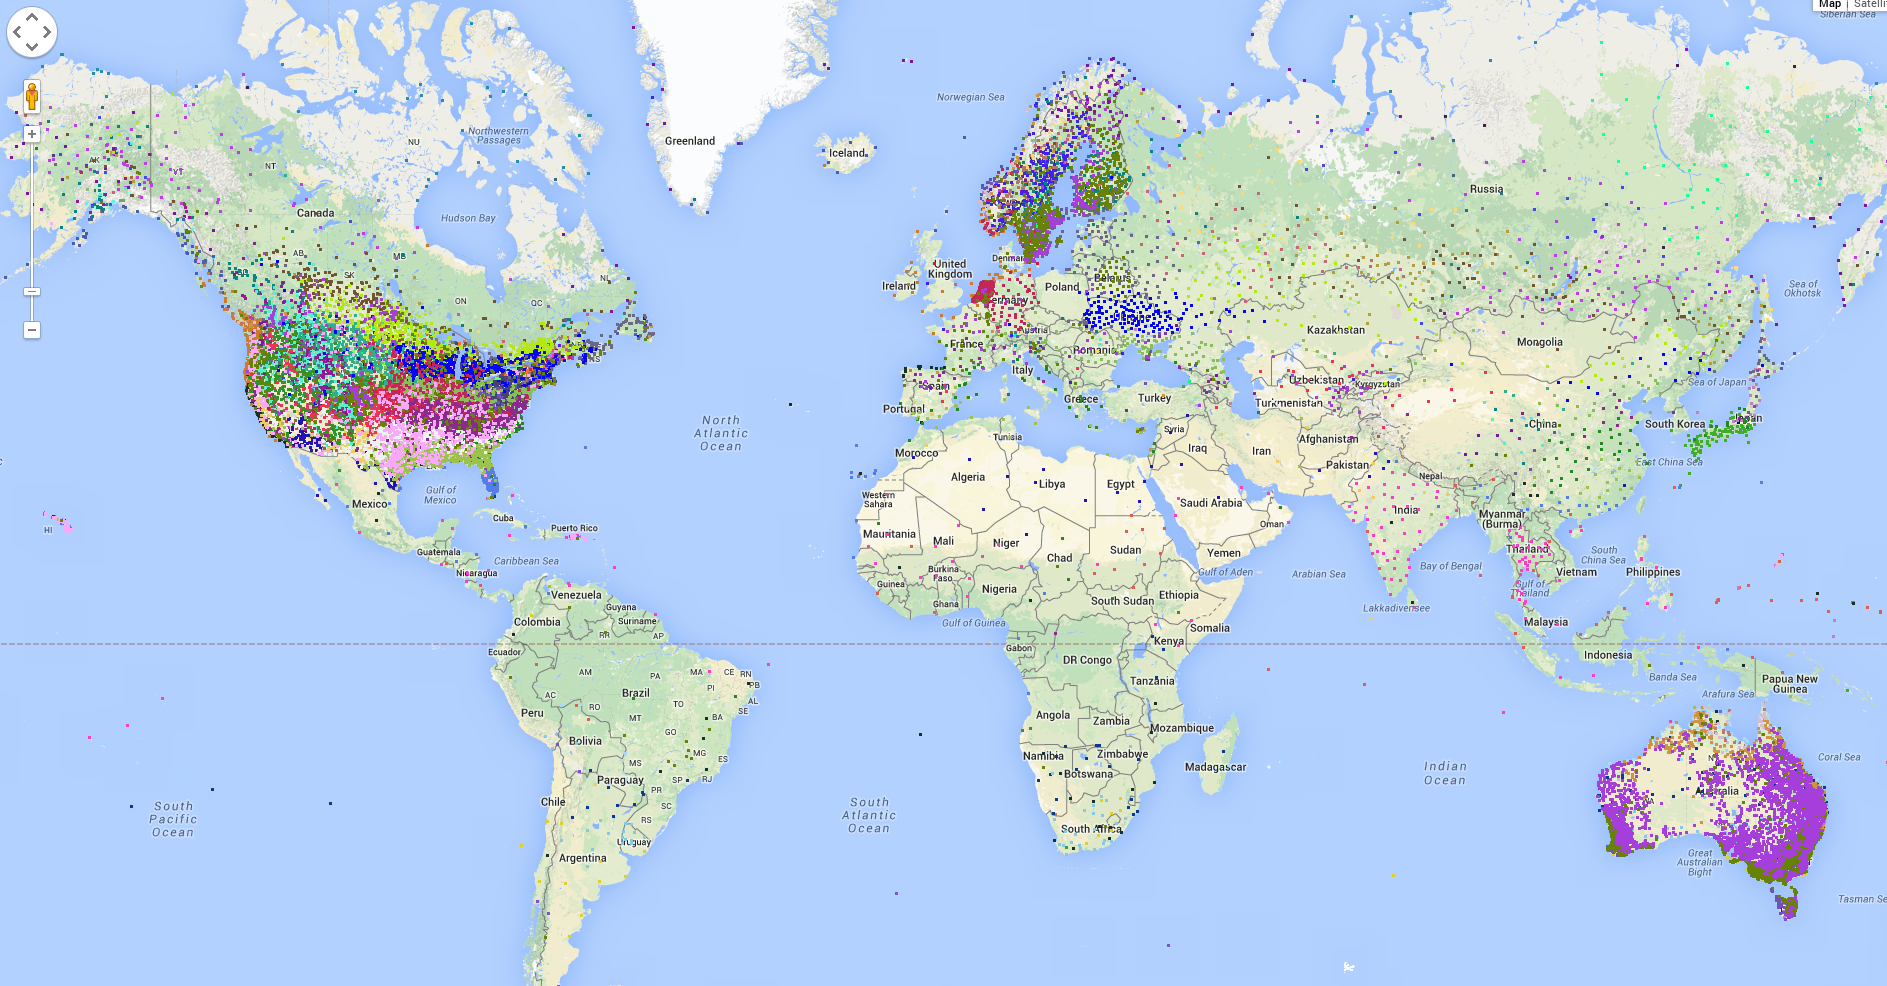
\includegraphics[width =\linewidth]{images/2003.png}\\2003\\
        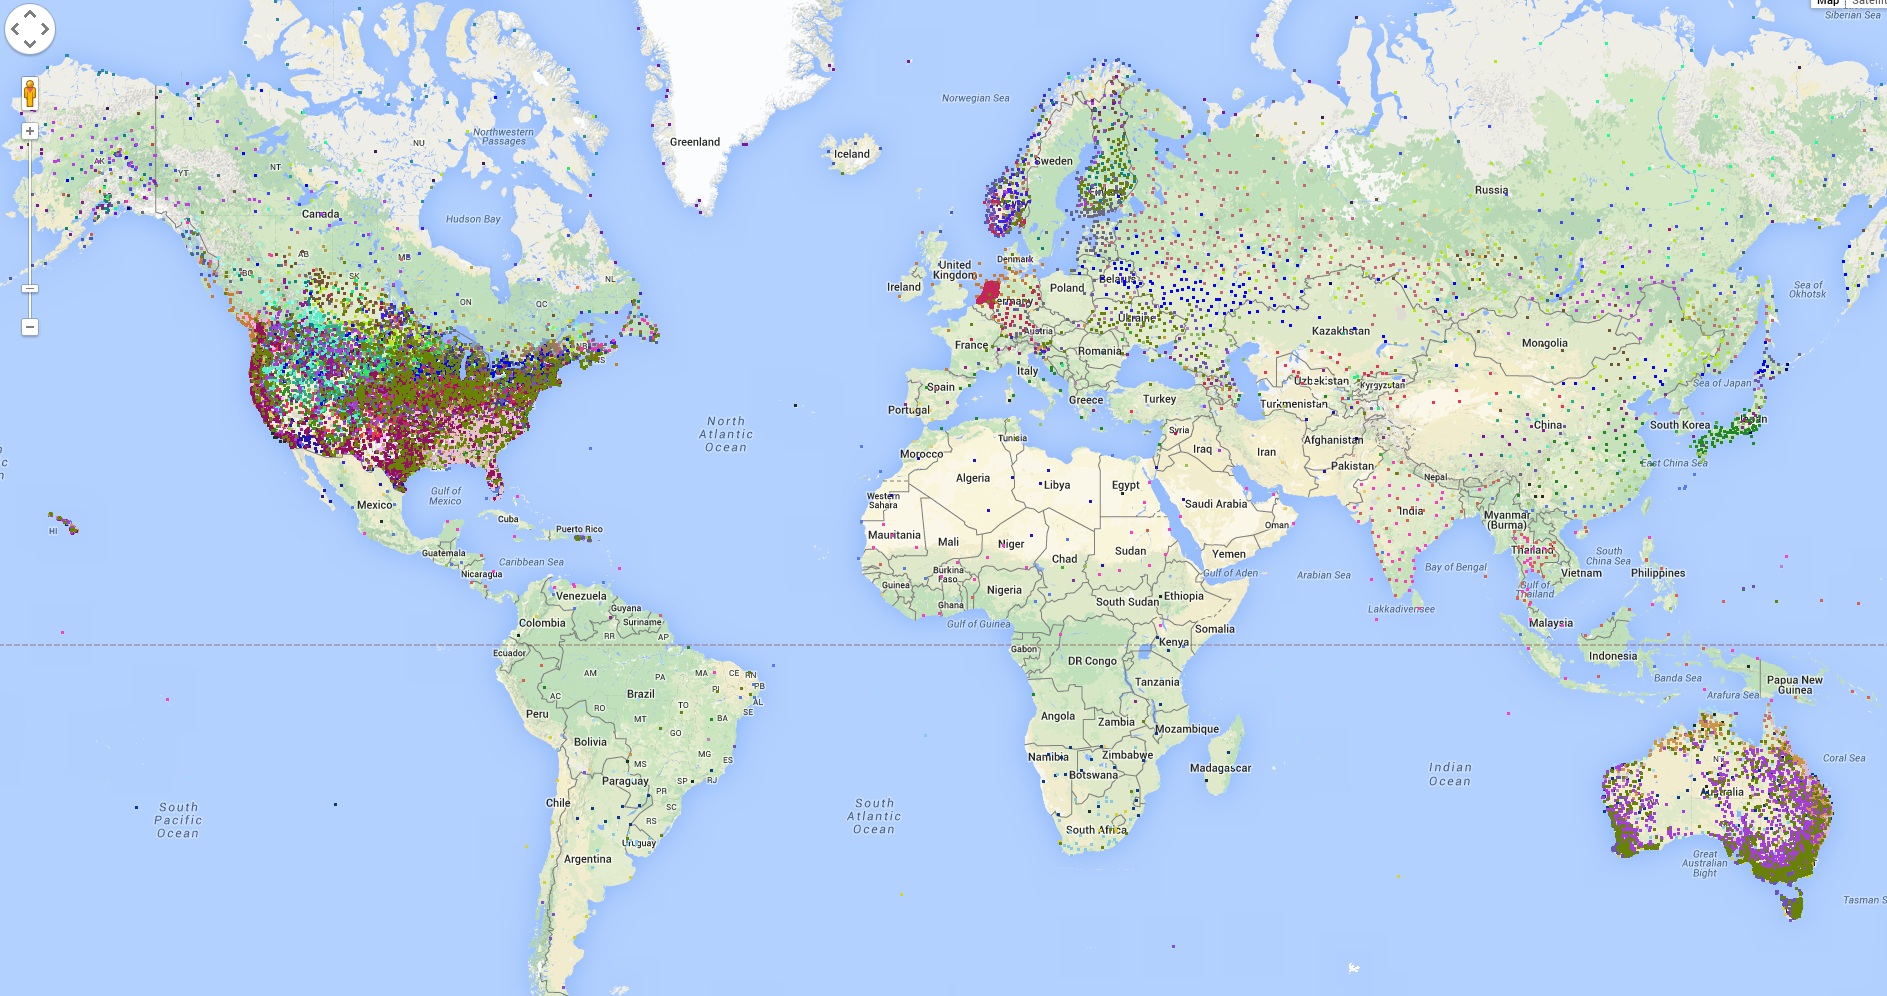
\includegraphics[width =\linewidth]{images/2013.png}\\2013\\
    \end{tabular}
    \caption{Clustering results of four different years.}
\end{figure}
\end{comment}

Compared with results in milestone $3$, there are two major improvements.
\begin{itemize}
    \item More clusters (which are different colors) are observed;
    \item Less mising points on the map;
\end{itemize}

\subsection{Result of more than a century}
Next, we adjusted the parameter again, when we run with $90$ clusters, $500$ iterations if there is any similar pattern to the extent of a century. We chose the years $1876$, $1896$, $1904$, $1940$, and $2010$ with the following size, so that the values are varying from $900K$ to $184M$.

\begin{table}
    \centering
    \begin{tabular}{|l|l|l|l|l|}
        \hline
        1876 & 1896 & 1904 & 1940 & 2010 \\
        \hline
        900K & 18M & 32M & 73M & 184M \\
        \hline
    \end{tabular}
\end{table}

The results before $1876$ is meaningless since there were not enough data.

\begin{comment}
\begin{figure}
    \centering
    \begin{tabular}{c}
        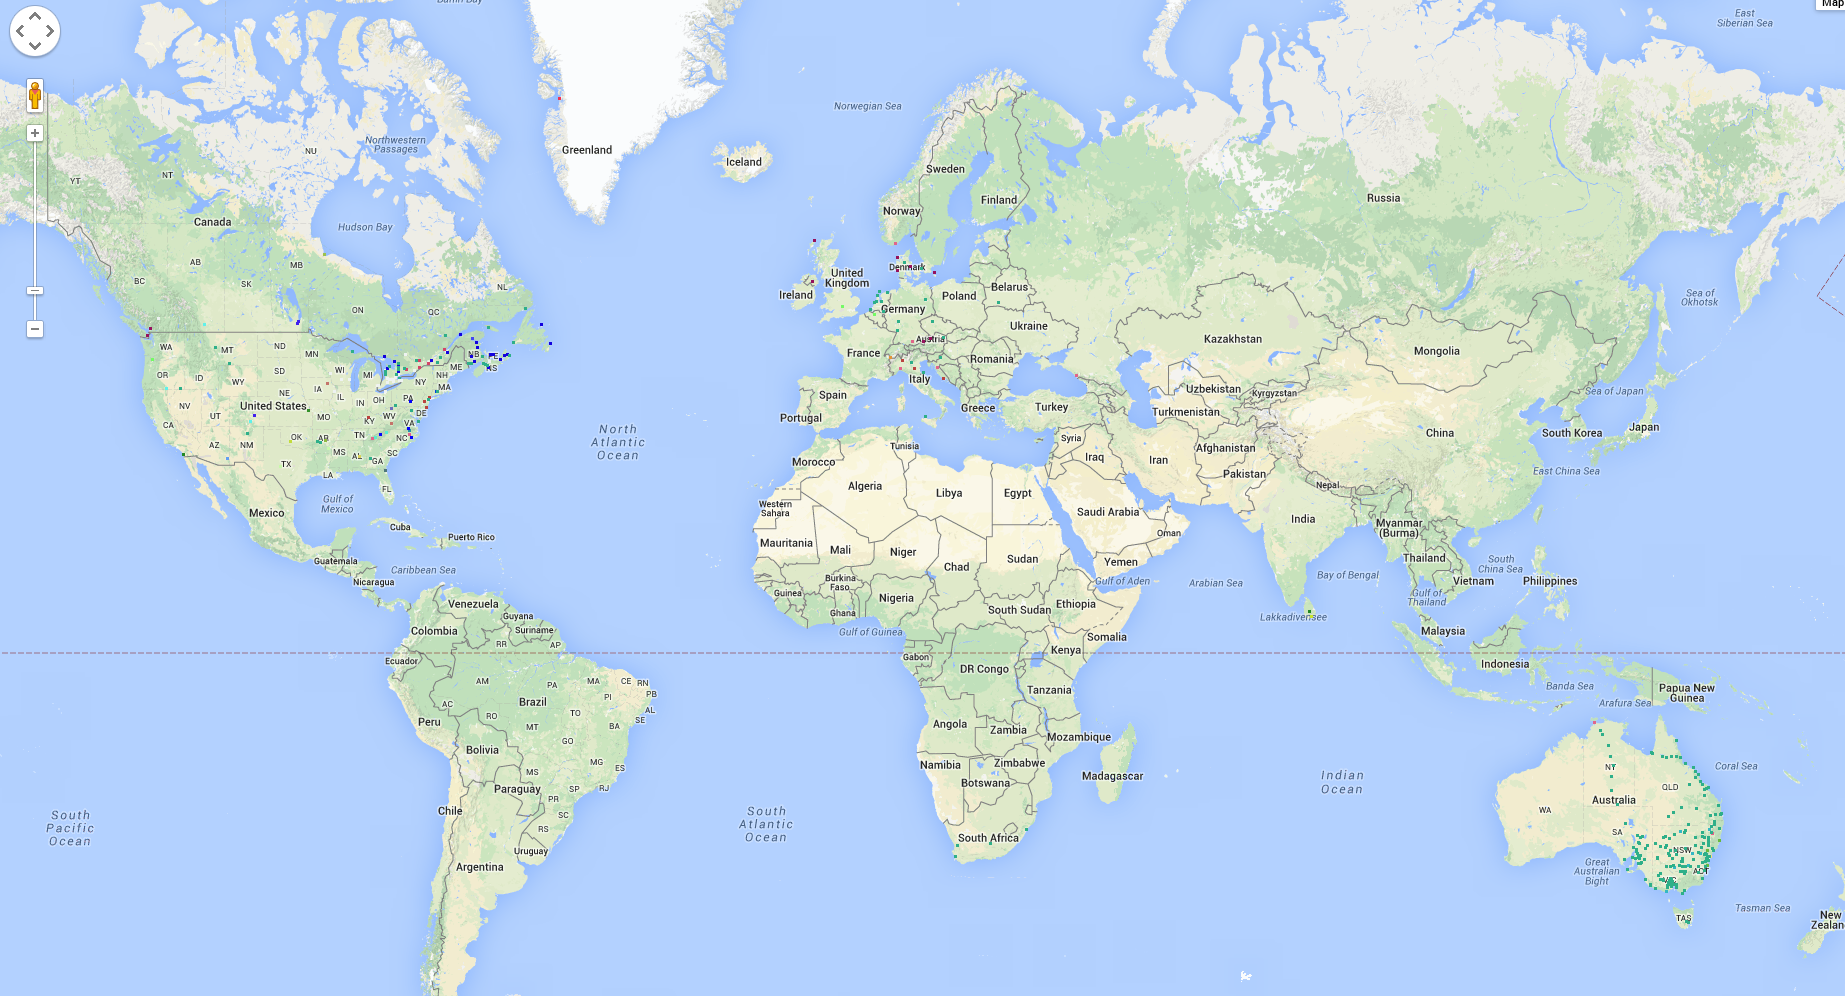
\includegraphics[width =.65\linewidth]{images/1876.png}\\ 1876\\
        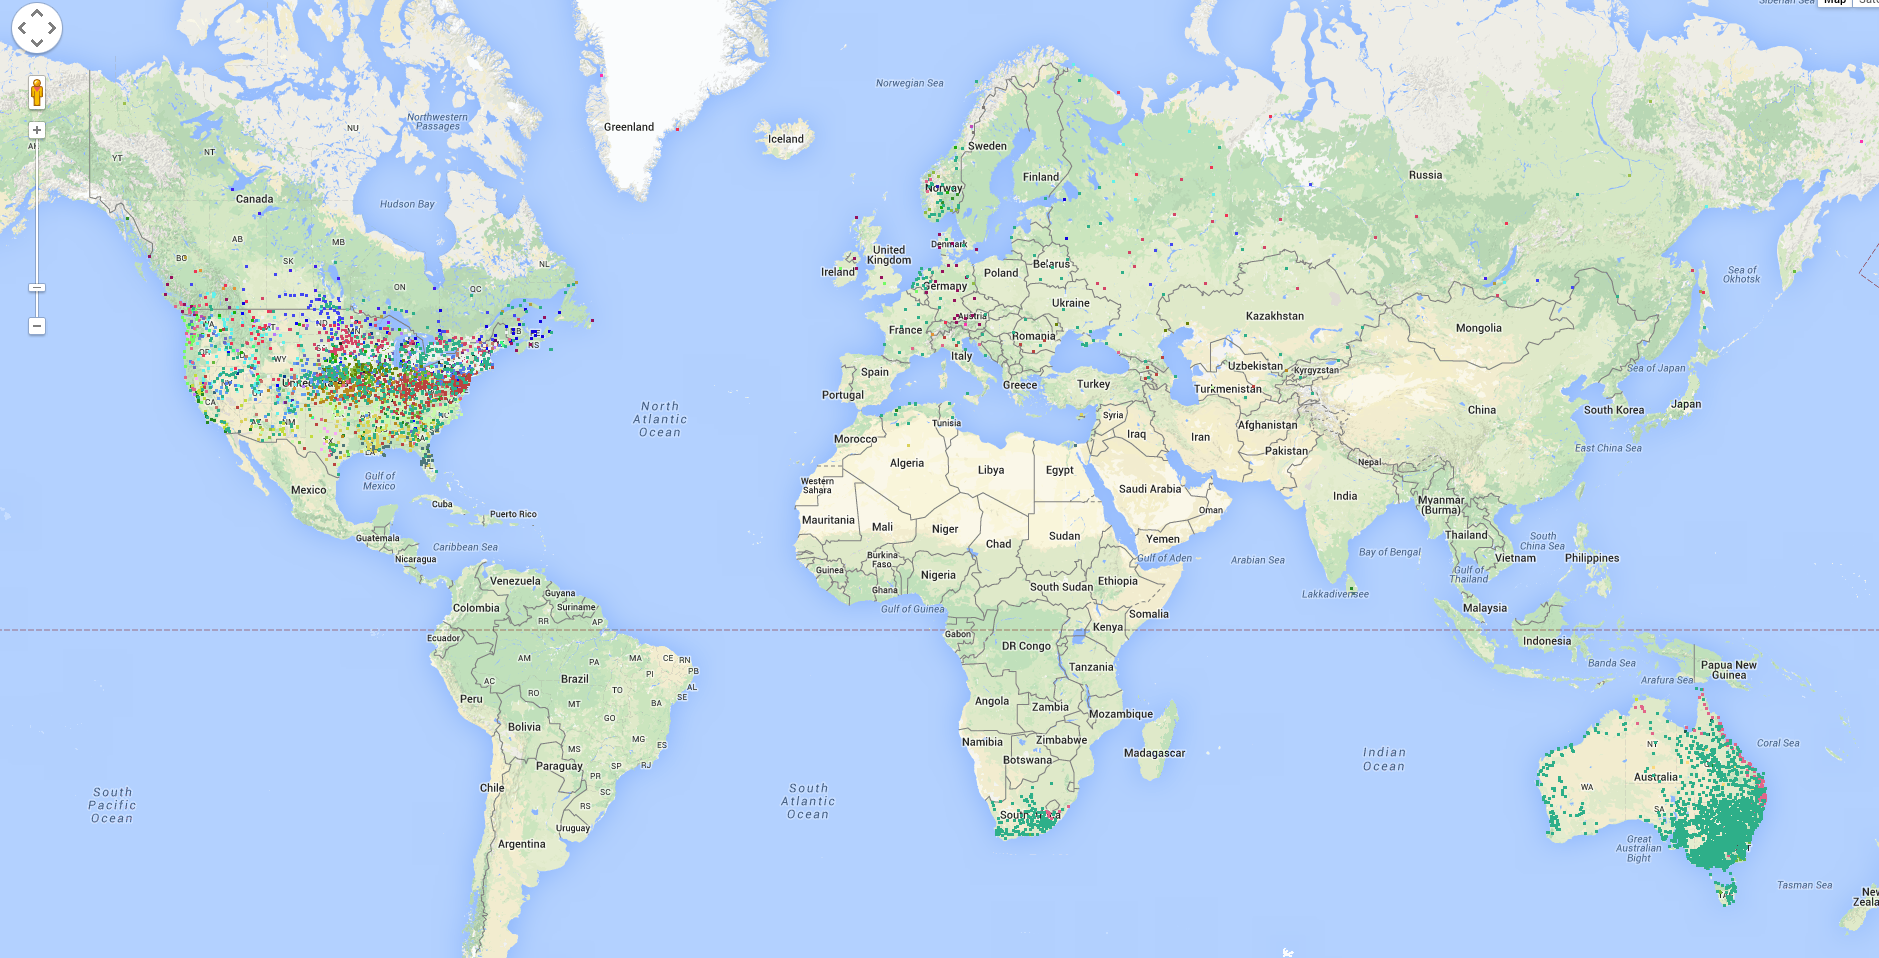
\includegraphics[width =.65\linewidth]{images/1896.png}\\ 1896\\
   \end{tabular}
    \caption{Clustering results over a century.}
\end{figure}
\begin{figure}
    \centering
    \begin{tabular}{c}
        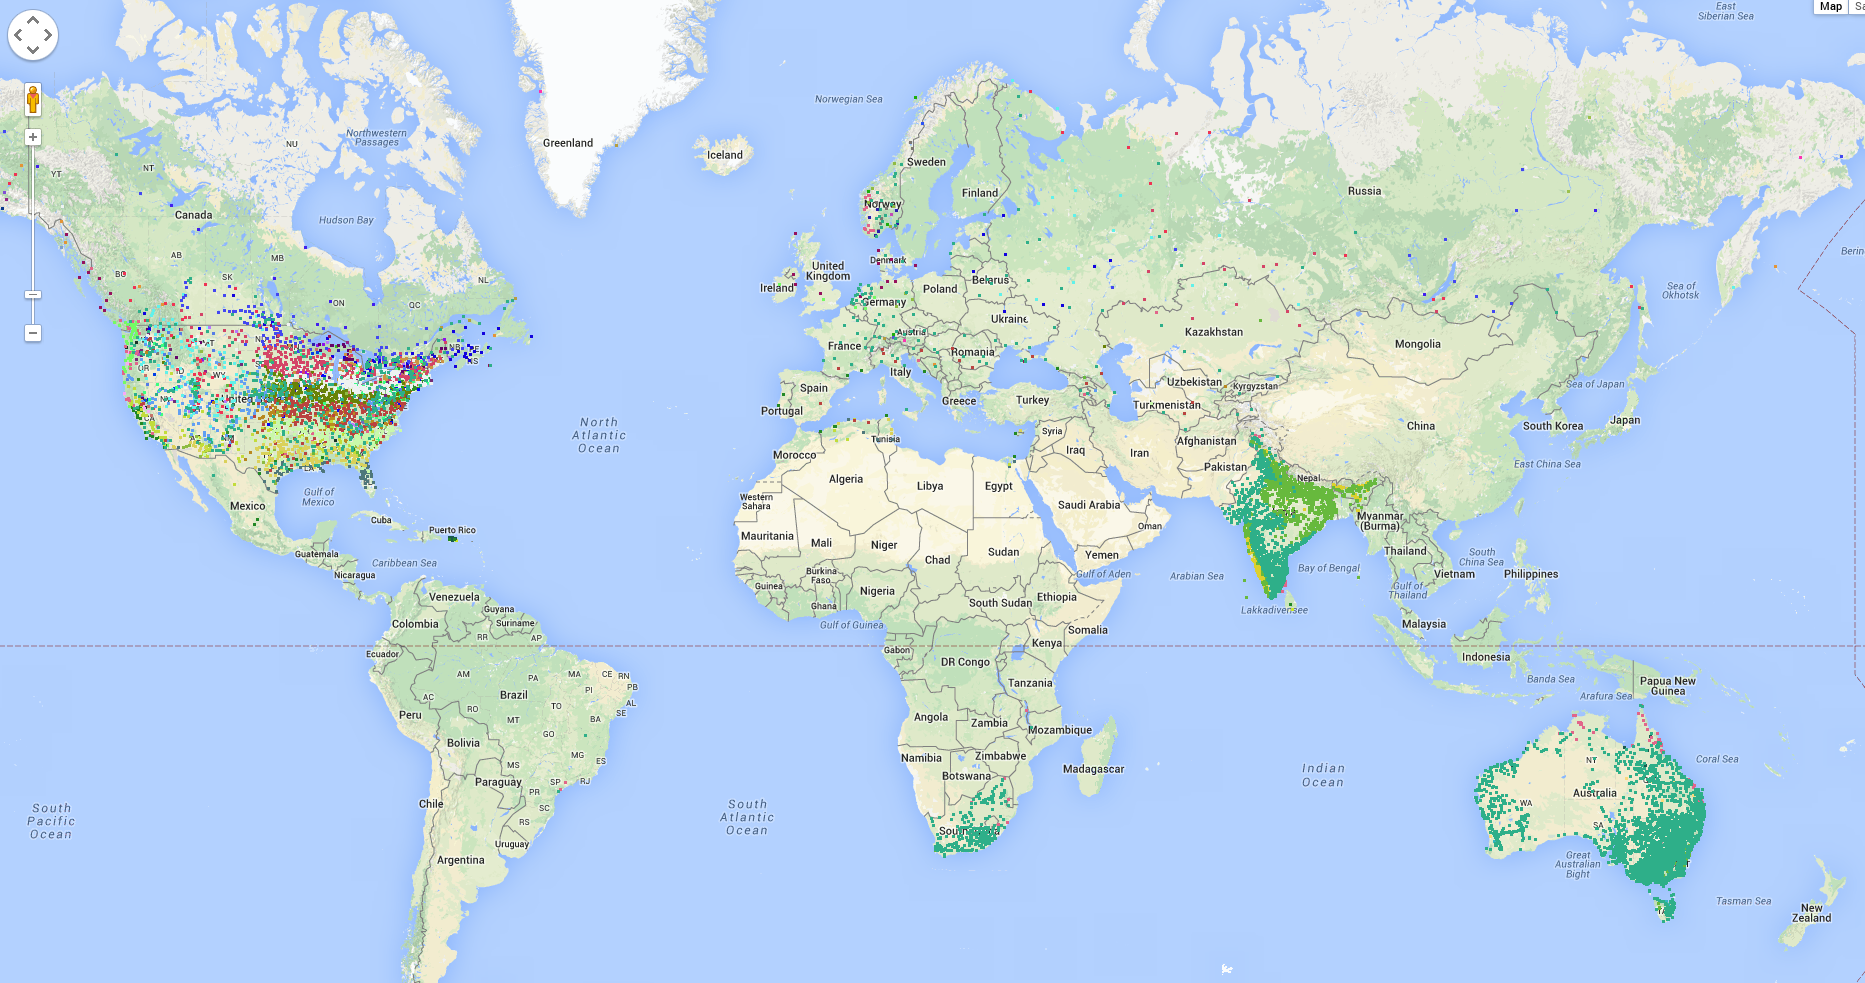
\includegraphics[width =\linewidth]{images/1904.png}\\ 1904\\
        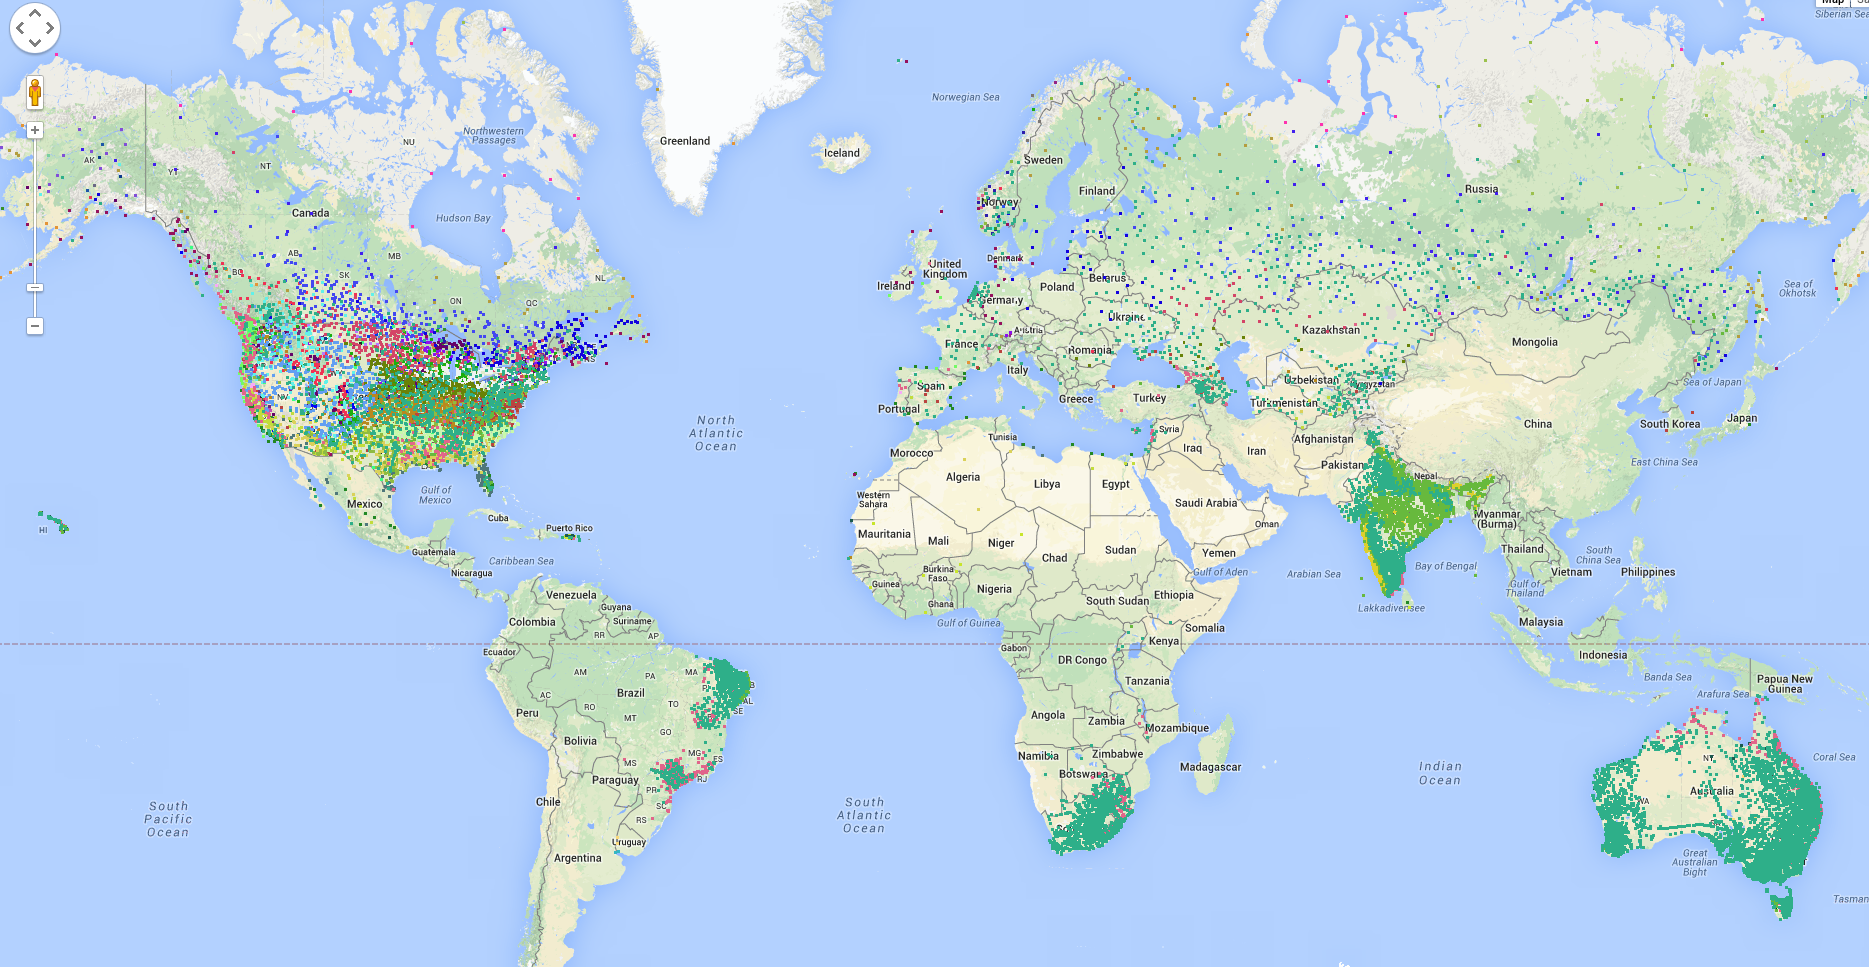
\includegraphics[width =\linewidth]{images/1940.png}\\ 1940\\
        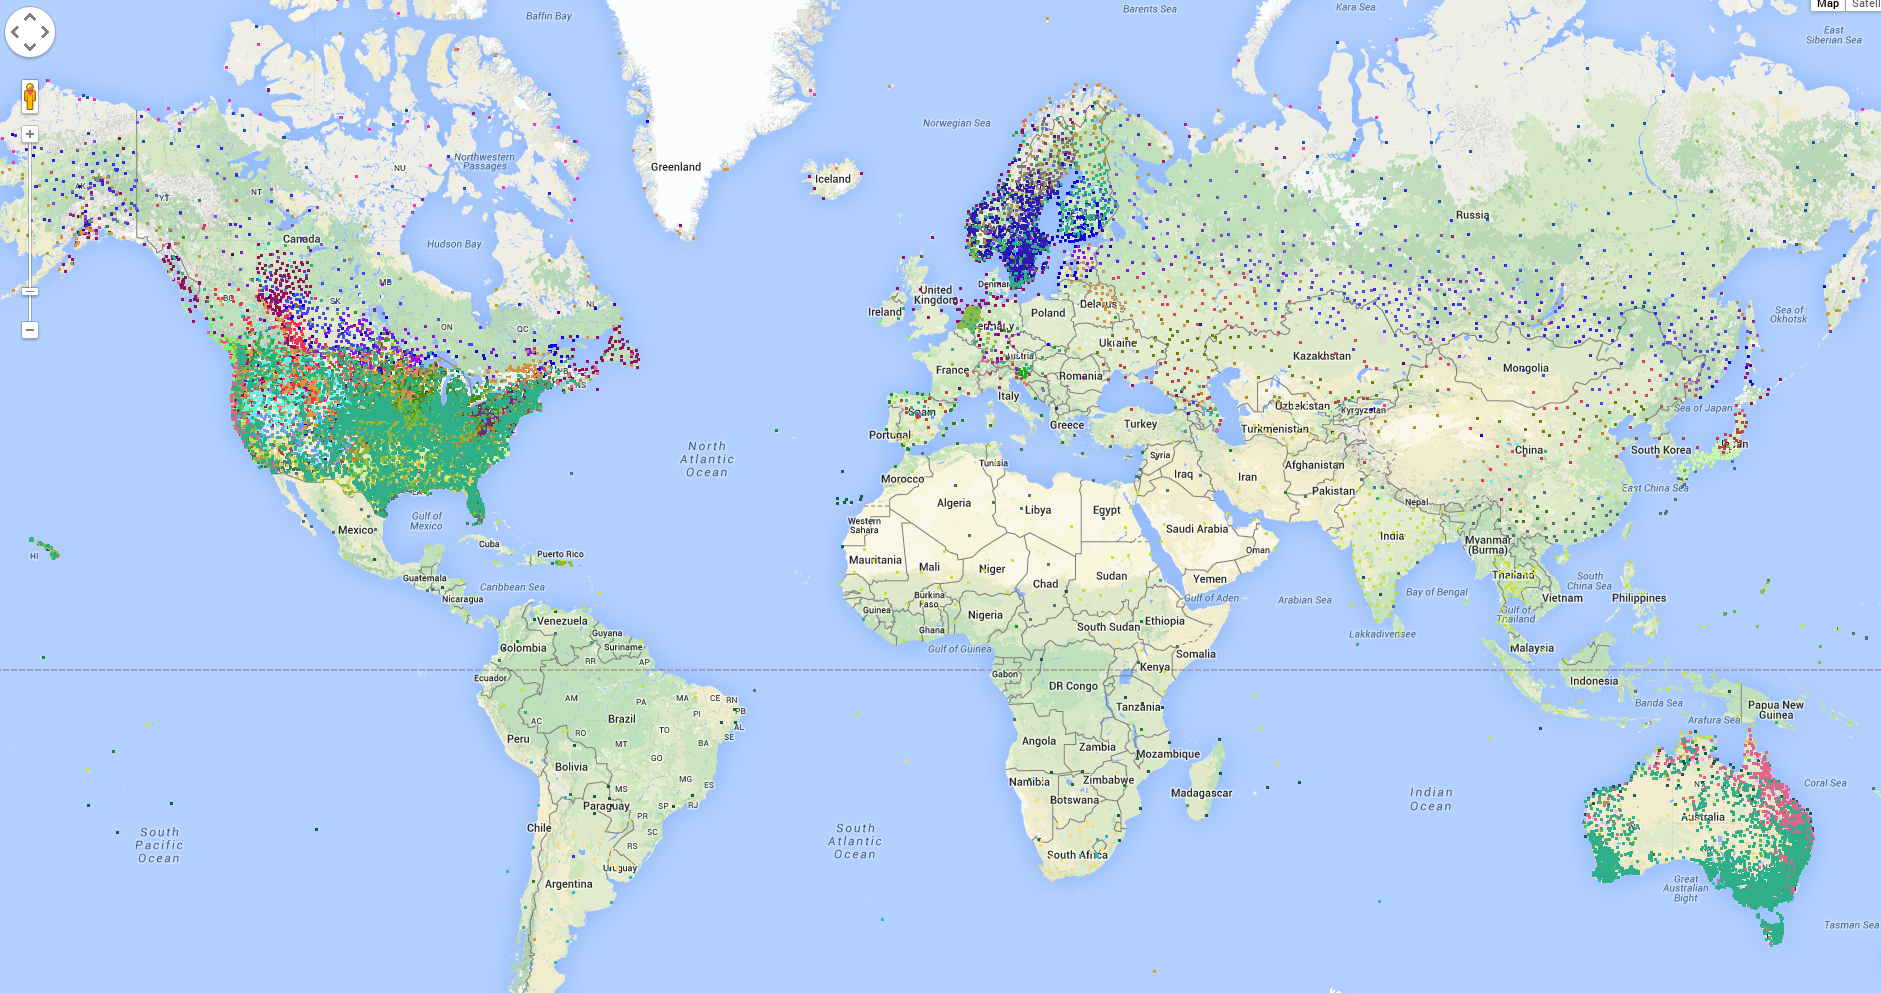
\includegraphics[width =\linewidth]{images/2010.png}\\ 2010\\
    \end{tabular}
\end{figure}
\end{comment}
 
\subsection{Result of recent $11$ years}
We extracted the result from $2003$ to $2013$, made a video by Python which is now available on Youtube.
